\chapter{Annexe 1 : Génération de l'App Bundle et l’APK en mode release}
\label{chap:annexe1}

Pour pouvoir générer l’\textbf{\gls{APK}} ou l'\textbf{App Bundle} en mode release, cliquez sur \textbf{Build} du menu horizontal d’Android Studio puis sur \textbf{Generate Signed Bundle/APK}. Une fenêtre s’ouvrira et vous serez demandé de choisir entre la génération d'App Bundle ou d’APK. Sélectionnez votre choix puis cliquez sur \textbf{Next}. Voir la première figure de \ref{Figure 7.1}. Dans la nouvelle fenêtre ouverte, cliquez sur \textbf{Create New} puis renseignez les informations demandées comme illustre la deuxième figure de \ref{Figure 7.1}.
\begin{figure}[!ht]
	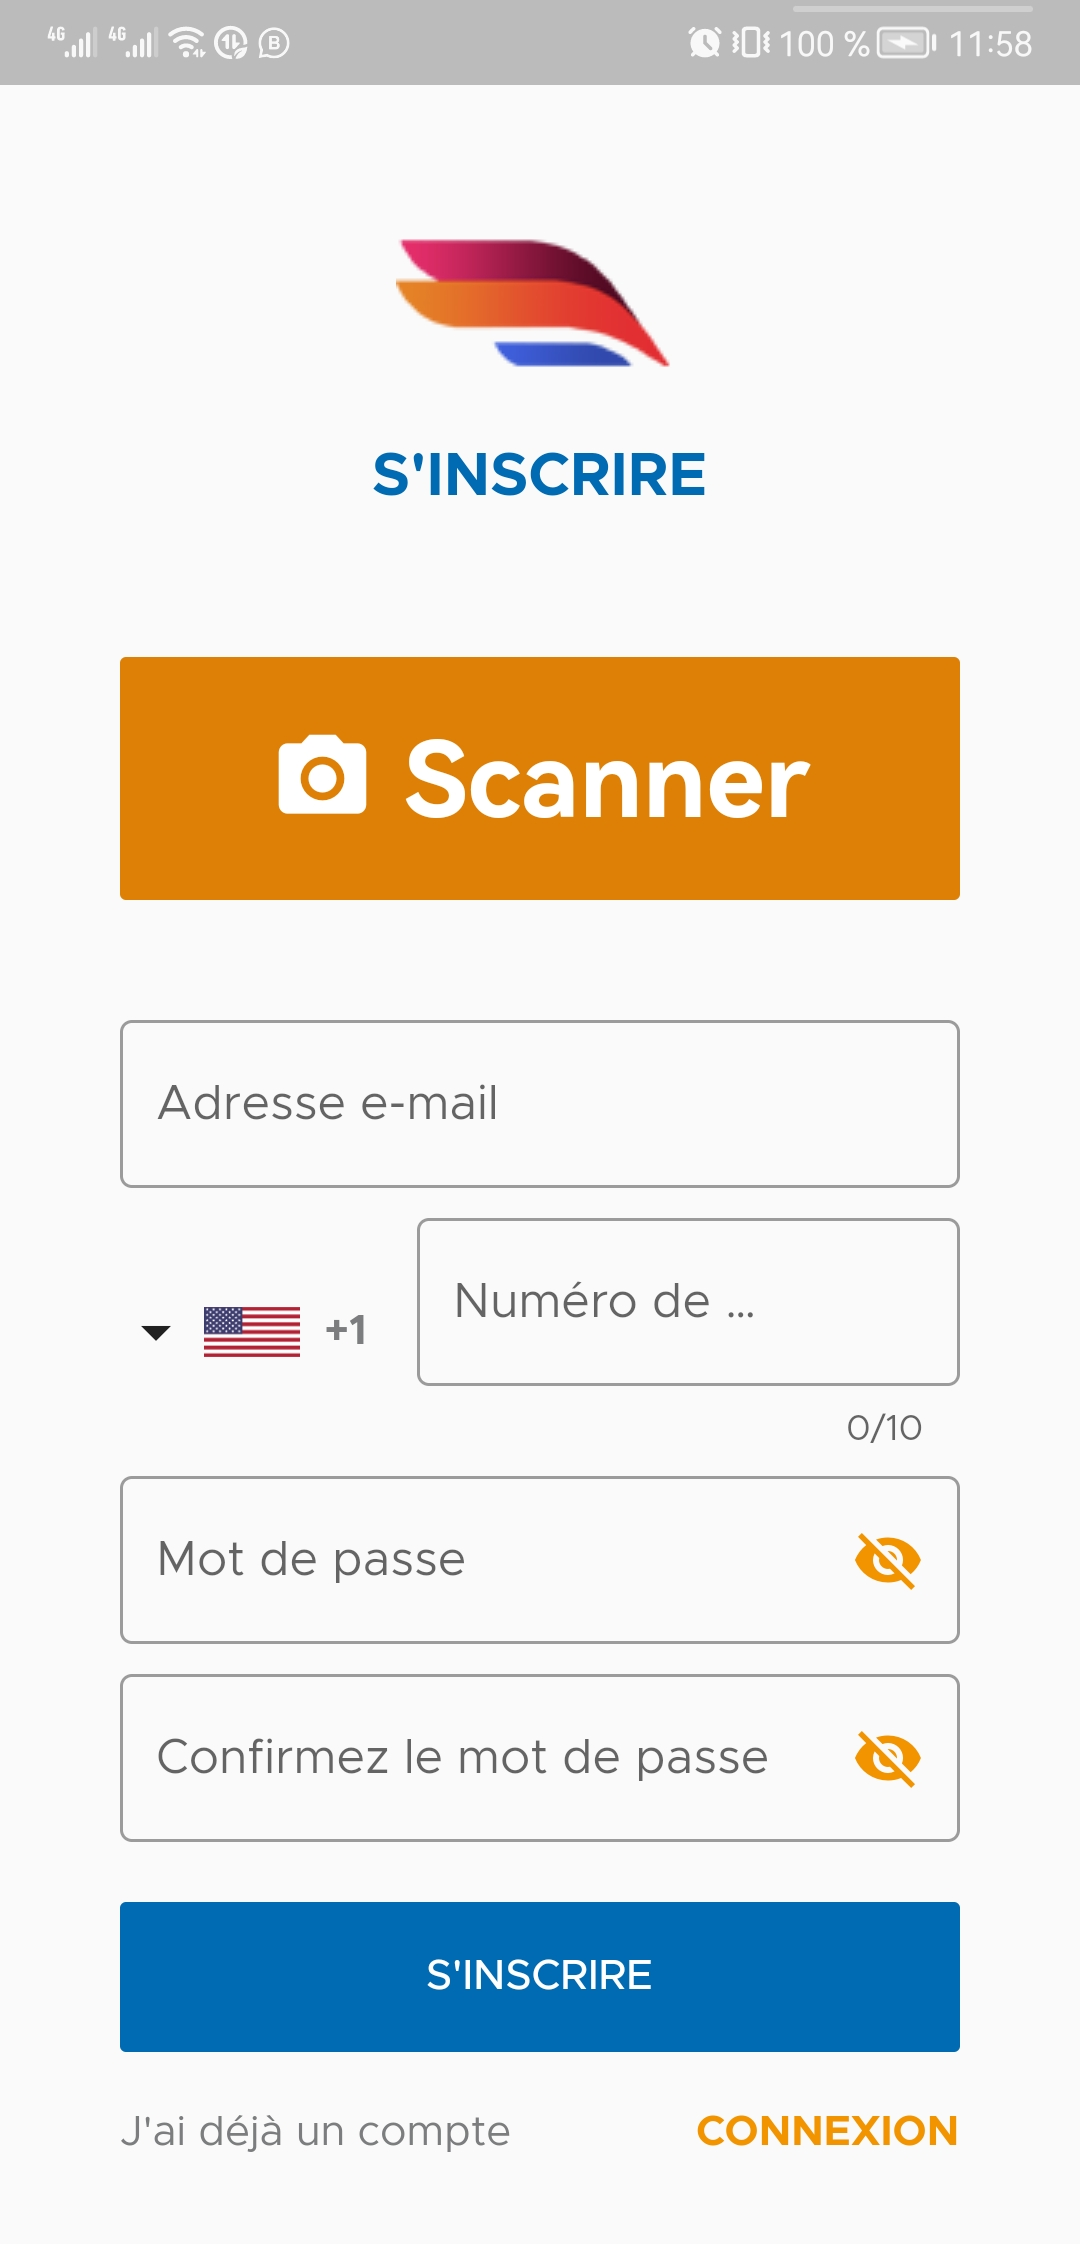
\includegraphics[scale=0.6]{D:/NTFS 3/Mon_master/M2/S4/Caputures_d_ecran_de_l_application/4}
	\includegraphics[scale=0.6]{D:/NTFS 3/Mon_master/M2/S4/Caputures_d_ecran_de_l_application/Capture}
	\centering
	\caption{Choix de génération et génération d’un nouveau Key Store.}
	\label{Figure 7.1}
\end{figure}
\newline Une fois cliqué sur \textbf{Ok}, vous aurez l’interface \ref{Figure 7.2} qui présente un aperçu sur l’ensemble des informations précédemment saisies.
\begin{figure}[!ht]
	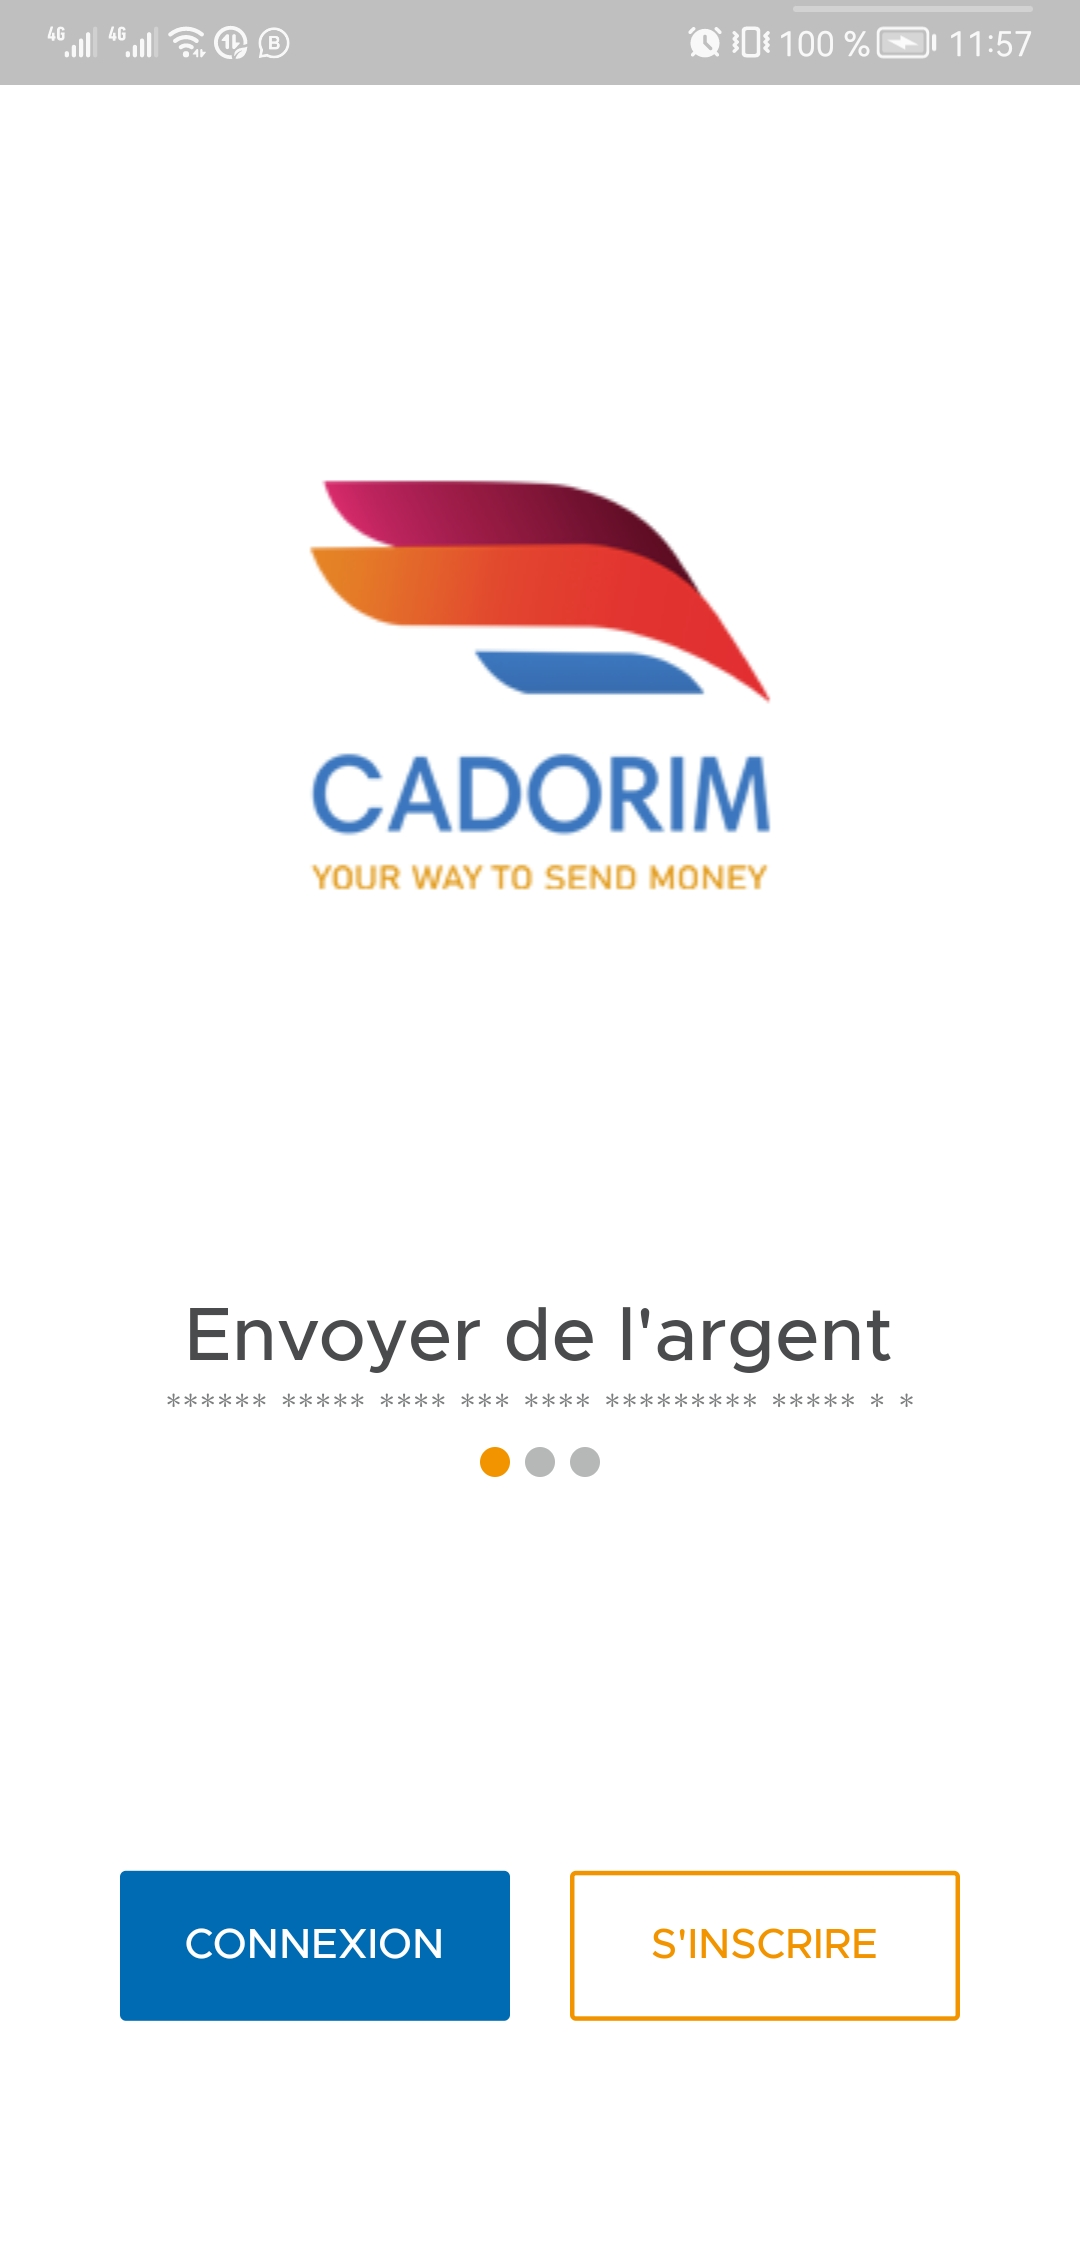
\includegraphics[scale=0.7]{D:/NTFS 3/Mon_master/M2/S4/Caputures_d_ecran_de_l_application/2}
	\centering
	\caption{Aperçu sur la configuration de l’APK ou de l'App Bundle.}
	\label{Figure 7.2}
\end{figure}
\newline Lorsque vous cliquez sur Next, vous aurez l’interface ci-dessous. Sélectionnez le mode release, puis cliquez sur Finish. La figure \ref{Figure 7.3} en présente une illustration.
\begin{figure}[!ht]
	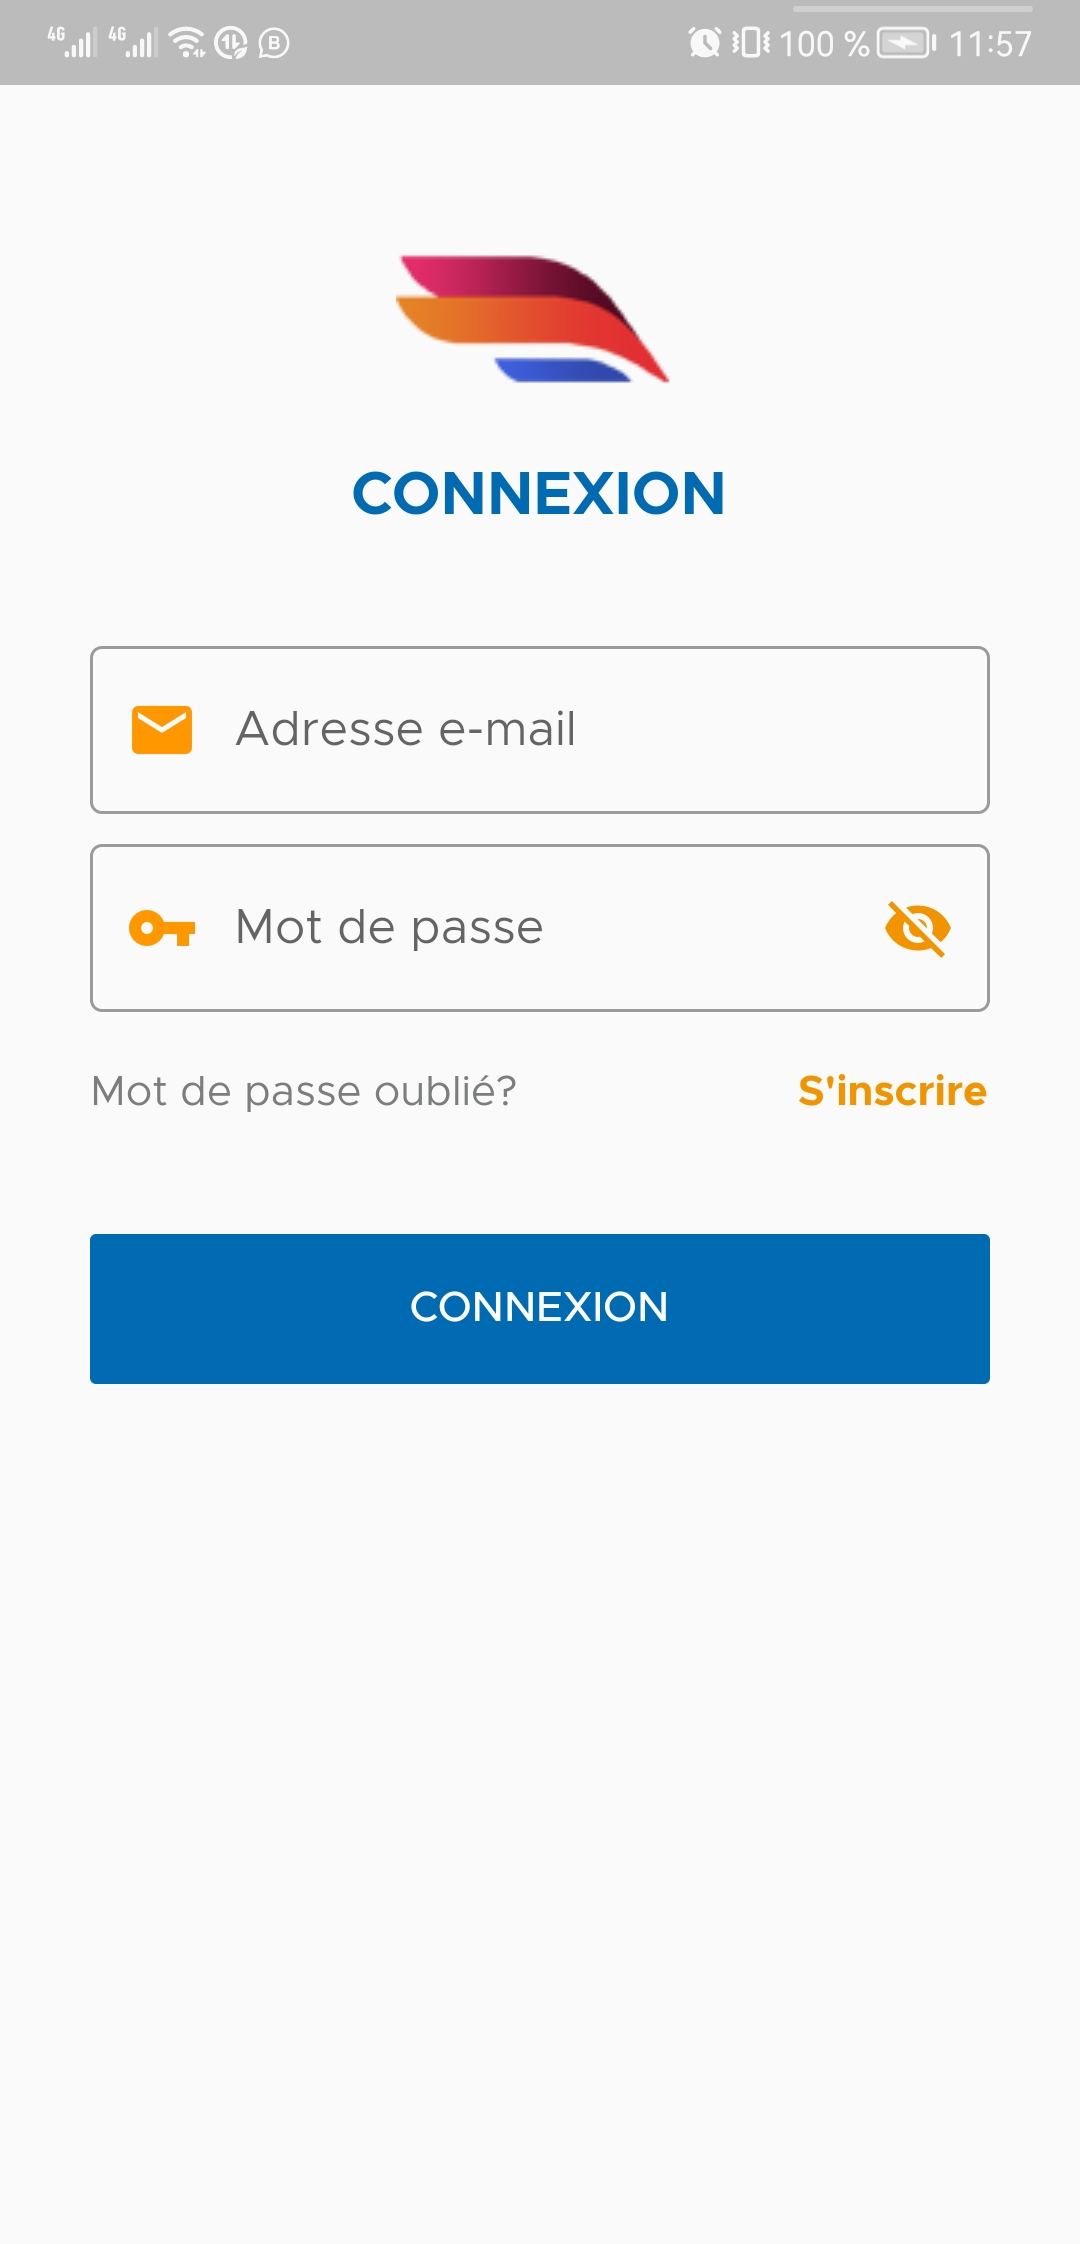
\includegraphics[scale=0.7]{D:/NTFS 3/Mon_master/M2/S4/Caputures_d_ecran_de_l_application/3}
	\centering
	\caption{Options de génération de l'App Bundle ou de l’APK en mode release.}
	\label{Figure 7.3}
\end{figure}
\newline Le processus de génération de l'App Bundle ou de l’APK peut durer quelques minutes suivant la performance de votre ordinateur. Une fois achevé, vous serez notifiez à ce propos. L'App Bundle ou l’APK généré en mode release se trouve dans /android/app/release du dossier du projet.